\chapter{Bounds on \(\mathbf{N}_{\text{patch}}\)}
\label{app:bounds}
\section{2D Green Function Approximation}
\label{app:2DGreenbounds}

Figures~\ref{fig:memoryTime2DGreenFused} and
\ref{fig:memoryTime2DGreenInterleaved} in
Chapter~\ref{chap:results} showed that a patched QTCI (pQTCI) run is advantageous only within a certain window of the patch bond–dimension cap
\(\chi_{\text{patch}}\).   To quantify that window we compare the measured patch count \(\mathcal
N_{\!p}\) with the theoretical bounds (cf. \prettyref{eq:chiPatchBound}) 

\begin{equation}
    \Np
    \;<\;
    \begin{cases}
      \displaystyle\chi^{2}/\chip^{2}, & \text{(memory)},\\[6pt]
      \displaystyle\chi^{3}/(d\,\chip^{3}), & \text{(CPU runtime)},
    \end{cases}
  \label{eq:chiPatchBoundApp}
\end{equation}
where \(\chi\) is the rank of the corresponding single–TT (standard QTCI)
approximation at the same discretisation parameters \((\mR,\tau)\).

For the pQTCI approximated function \(\operatorname{Re}G(\bk)\) [\prettyref{eq:2DGreen}] we plot \(\Np-\bigl(\chi^{2}/\chi_{\text{patch}}^{2}\bigr)\) and
\(\Np-\bigl[\chi^{3}/(d\,\chip^{3})\bigr]\) for
selected \((\delta)\) values and index unfoldings.   Negative values mean that the bound is not correctly satified.

\begin{figure}[htpb]
    \centering
    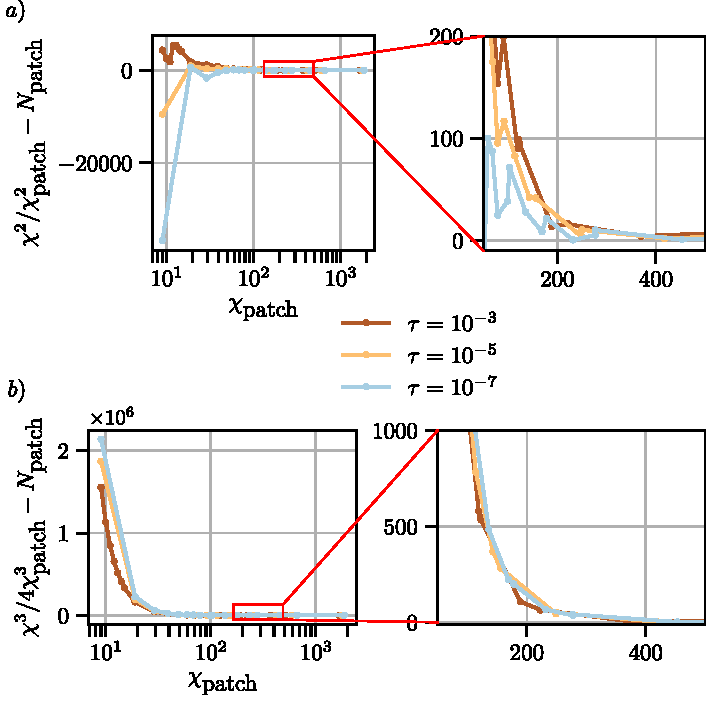
\includegraphics{figures/2DGreenMemoryTimeBoundFused.pdf}
    \caption{\textbf{Fused ordering, \(\delta=10^{-3}\).}
    Difference between the actual patch count \(\Np\) and the memory (a) and run–time (b) bounds of \prettyref{eq:chiPatchBoundApp}.
    Negative values indicate that the bound is not respected.}
    \label{fig:memoryBound2GreenFused}
\end{figure}

\begin{figure}[htpb]
    \centering
    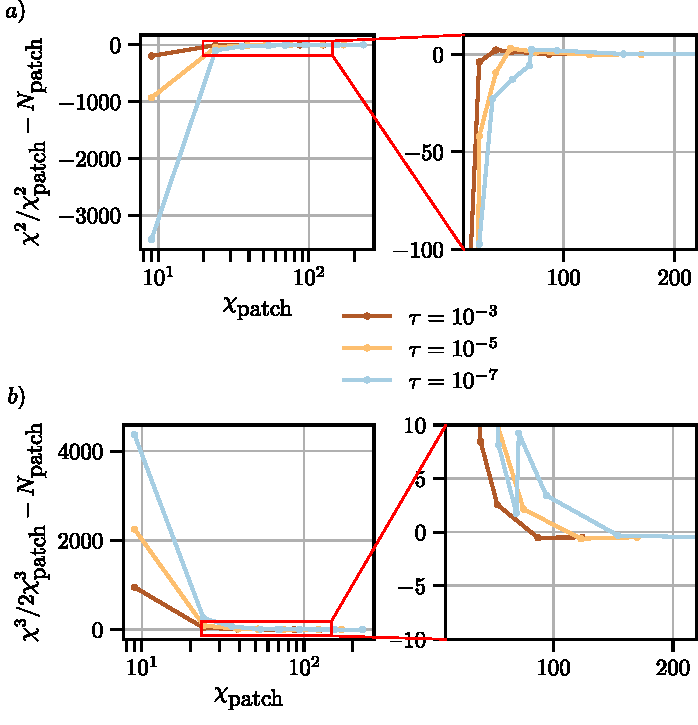
\includegraphics{figures/2DGreenMemoryTimeMemoryBoundInterleaved.pdf}
    \caption{\textbf{Interleaved ordering, \(\delta=10^{-1}\).}
    Same analysis as Fig.~\ref{fig:memoryBound2GreenFused}.
    Here pQTCI tends to \emph{violate} the bounds more often because \(\operatorname{Re}G(\bk)\) is already smooth and the algorithm over–patches the domain.}
    \label{fig:memoryBound2GreenInterleaved}
\end{figure}

Several trends emerge:

\begin{itemize}
  \item For sharp spectral lines (\(\delta=10^{-3}\), fused ordering,
        Fig.~\ref{fig:memoryBound2GreenFused}) the bounds are comfortably
        met in the optimum \(\chi_{\text{patch}}\) range, explaining the
        clear savings seen in Fig.~\ref{fig:memoryTime2DGreenFused}.
  \item When the Green’s function is broad (\(\delta=10^{-1}\), interleaved
        ordering, Fig.~\ref{fig:memoryBound2GreenInterleaved}) the algorithm
        slices the domain more than necessary; the patch count exceeds the
        theoretical limits and the patched run is no longer profitable.
  \item Although Fig.~\ref{fig:memoryTime2DGreenFused} shows time savings
        only at specific \(\chi_{\text{patch}}\), the run–time bound in
        Eq.~\eqref{eq:chiPatchBoundApp} is \emph{always} satisfied.  The
        apparent discrepancy could be due to the current pQTCI implementation, whose task–scheduling overhead masks the benefit except when the single–TT contraction becomes truly expensive. Moreover, the bounds are only an rough estimates. Many more variables play a role in the actual runtime of the implemented pQTCI algorithm
\end{itemize}

In summary, the bounds of \prettyref{eq:chiPatchBoundApp} provide a somewhat reliable
indicator of when pQTCI will outperform a monolithic QTCI run: the algorithm is advantageous around the parameter regions where both the memory and time inequalities are fulfilled.

\section{Patched MPO-MPO contractions}
\label{sec:PatchContrbounds}
\subsection{Matrix muliplication}
The limits derived in \prettyref{eq:worstBound}, \prettyref{eq:bestBound}, and \prettyref{eq:averageBound} assume that the
two MPO factors share the same patching depth~\(\bar\ell\).  If the left MPO \(\widetilde{\mF}_{\bsigma,\bsigma'}\) and the right MPO
\(\widetilde{\mG}_{\bsigma',\bsigma''}\) are patched to \emph{different} levels, the bounds depend onf both of their patch numbers. With \(\chi_{\mF}\) and \(\chi_{\mG}\) denoting the bond dimensions of the corresponding non-patched tensors, and \(\chi_{\text{patch},\mF}\), \(\chi_{\text{patch},\mG}\) the caps imposed on each factor, the generalised conditions read

\begingroup
\renewcommand{\labelenumi}{(\alph{enumi})}
    \begin{enumerate}
        \item \textbf{Worst case}
        \begin{equation}
          N_{\text{patch},\mF}N_{\text{patch},\mG}
    <\frac{\chi^2_{\mF}\chi^2_{\mG}}{\chi^2_{\text{patch},\mF}\chi^2_{\text{patch},\mG}}
            \label{eq:newworstBoundApp}
        \end{equation}
      \item \textbf{Best case}
        \begin{equation}
          \Np^{\text{max}}
    <\frac{\chi^2_{\mF}\chi^2_{\mG}}{\chi^2_{\text{patch},\mF}\chi^2_{\text{patch},\mG}} 
            \label{eq:newbestBoundApp}
        \end{equation}
      where $\Np^{\text{max}} = \max \{N_{\text{patch},\mF},N_{\text{patch},\mG}\}$.

     \item \textbf{Average case} Let \(\bar\ell_{\min}\) be the smaller and \(\bar\ell_{\max}\) the larger patching level for the two factors.  The number of admissible patch pairs is \(d^{\bar\ell_{\min}}d^{\bar\ell_{\min}(D-1)/D}d^{\bar\ell_{\max}-\bar\ell_{\min}}\) (cf. \prettyref{eq:averageBound}), leading to
        \begin{equation}
          N^{\frac{D-1}{D}}_{\text{patch},\mF}N_{\text{patch},\mG}\
    <\frac{\chi^2_{\mF}\chi^2_{\mG}}{\chi^2_{\text{patch},\mF}\chi^2_{\text{patch},\mG}}.
            \label{eq:newaverageBoundApp}
        \end{equation}
    \end{enumerate}
\endgroup
This bounds can be tested for the results we showed in \prettyref{fig:patchedMulResults}. For each data point of the \textit{worst-case}, \textit{best-case} and \textit{average-case} scenario we subtract the r.h.s. and the l.h.s. of the inequalities in \prettyref{eq:newworstBoundApp}, \prettyref{eq:newbestBoundApp} and \prettyref{eq:newaverageBoundApp}, respectively, and plot the resulting ``bound difference'' in \prettyref{fig:patchedMulBounds}. We observe an approximate correspondence between the ``overpatched'' runs in \prettyref{fig:patchedMulResults} and negative ``bound difference''. In particular, no data point in the \textit{worst-case-scenario} satisfies the bound, while most of the \textit{best-case-scenario} runs do.

\begin{figure}[htpb]
    \centering
    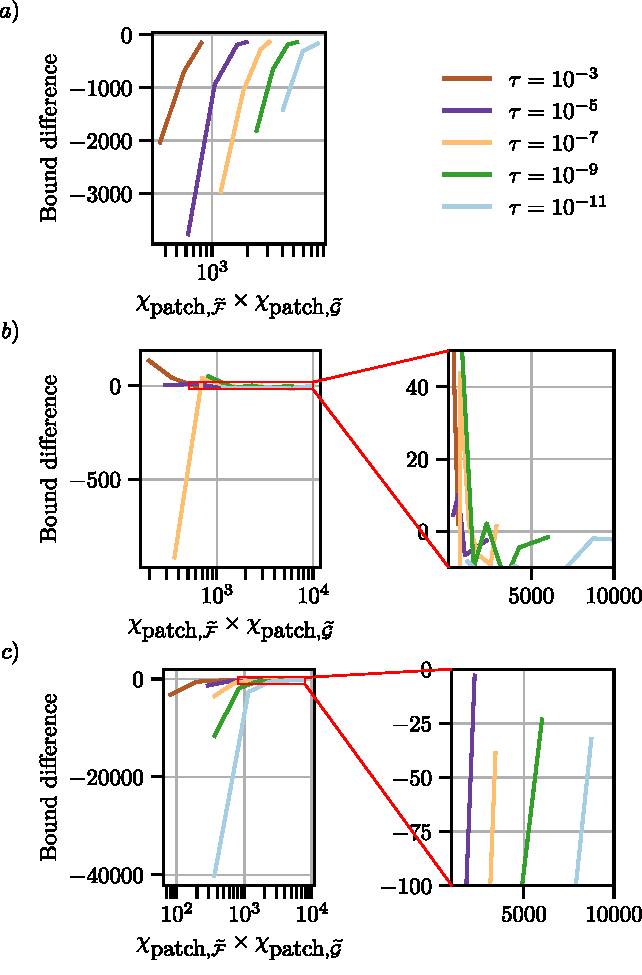
\includegraphics{figures/patchedMulBounds.pdf}
    \caption{Deviation of the measured number of patch products from the theoretical limits of Eqs.~\eqref{eq:newworstBoundApp}, \eqref{eq:newbestBoundApp}, and \eqref{eq:newaverageBoundApp}. Negative values indicate that the bound is \emph{not} satisfied. We illustrate the \textit{worst} $(a)$, \textit{best} $(b)$ and \textit{average} $(c)$ case patche MPO-MPO contraction bounds.}
    \label{fig:patchedMulBounds}
\end{figure}



Irrespective of the simulation parameters ($\tau$, $\mR$), the total number of floating-point entries in the result tensor, as measure of the contraction complexity, obeys 
\begingroup
\renewcommand{\labelenumi}{(\alph{enumi})}
    \begin{enumerate}
        \item \textbf{Worst case}
        \begin{equation}
          \order \bigl( N_{\text{patch},\mF}N_{\text{patch},\mG} \chi^2_{\text{patch},\mF}\chi^2_{\text{patch},\mG} \bigr).
            \label{eq:newworstScalingApp}
        \end{equation}
      \item \textbf{Best case}
        \begin{equation}
          \order \bigl( N_{\text{patch},\text{max}}N_{\text{patch},\mG} \chi^2_{\text{patch},\mF}\chi^2_{\text{patch},\mG} \bigr). 
            \label{eq:newbestScalingApp}
        \end{equation}

     \item \textbf{Average case}
     \begin{equation}
          \order \bigl( N^{\frac{D}{D-1}}_{\text{patch},\mF}N_{\text{patch},\mG} \chi^2_{\text{patch},\mF}\chi^2_{\text{patch},\mG} \bigr).
          \label{eq:newaverageScalingApp}
      \end{equation}
    \end{enumerate}
\endgroup

\prettyref{fig:patchedMulMemoryScaling} confirms these scaling laws: the measured parameter counts collapse onto the predicted combinations of \(N_{\text{patch}}\) and \(\chi_{\text{patch}}\) for the two factors $\mF$ and $\mG$.

\begin{figure}[htpb]
    \centering
    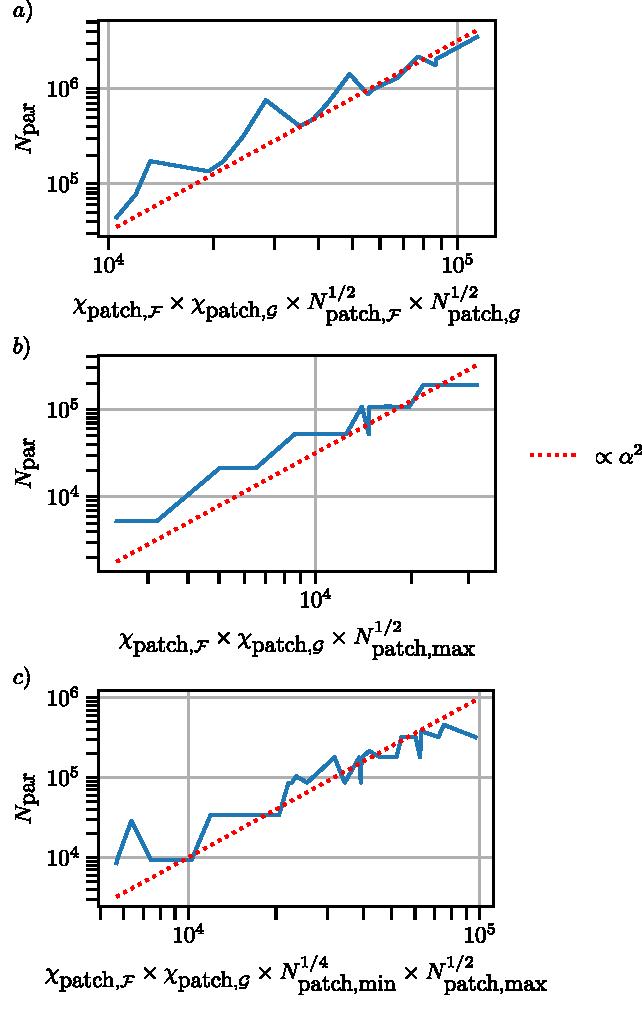
\includegraphics{figures/patchedMulMemoryScaling.pdf}
    \caption{Total number of parameters in set of patches representing \(\mathcal H\) versus the scaling variables from Eqs.~\eqref{eq:newworstScalingApp}–
           \eqref{eq:newaverageScalingApp}.  Solid lines illustrate data; dotted lines are the expected
           theoretical trends.}
    \label{fig:patchedMulMemoryScaling}
\end{figure}


\subsection{Element-wise multiplication}
For an element–wise product of two tensors
\(\mF_{\bsigma}\) and \(\mG_{\bsigma}\) the patch–count limit of Eq.~\eqref{eq:elemMulBound} generalises to
\begin{equation}
          \Np^{\text{max}}
    <\frac{\chi^2_{\mF}\chi^2_{\mG}}{\chi^2_{\text{patch},\mF}\chi^2_{\text{patch},\mG}} 
            \label{eq:newElemBoundApp}
        \end{equation}
where $\Np^{\text{max}} = \max \{N_{\text{patch},\mF},N_{\text{patch},\mG}\}$. \prettyref{fig:elemMulBounds} plots the difference between the left– and right–hand sides for all data points of \prettyref{fig:elemMulResults}.  
Negative bars mark those instances where the patched run exceeds the bound.

\begin{figure}[htpb]
    \centering
    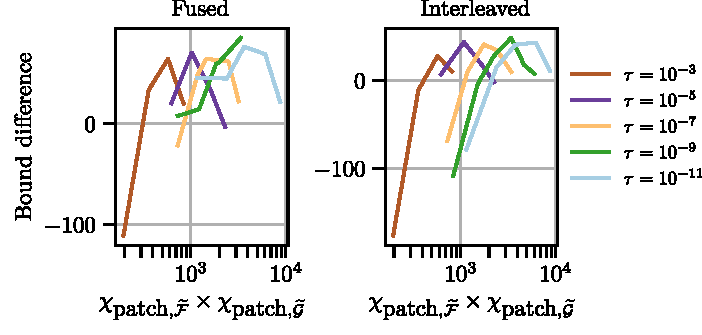
\includegraphics{figures/elemMulBounds.pdf}
    \caption{Deviation from the bound
           in Eq.~\eqref{eq:newElemBoundApp} for element-wise
           multiplication of \(\mF_{\bsigma}\) and \(\mG_{\bsigma}\).
           Separate series are shown for fused and interleaved index
           orderings.  Negative values indicate a violation of the bound.}
    \label{fig:elemMulBounds}
\end{figure}

As measure of contraction complexity, the total number of floating-point parameters in the patched product should scale as

\begin{equation}
  \mathcal{O} \bigl(
    N_{\text{patch},\max}\,
    N_{\text{patch},\min}\,
    \chi_{\text{patch},\mF}^{2}\,
    \chi_{\text{patch},\mG}^{2}
  \bigr),
  \label{eq:newElemScalingApp}
\end{equation}

with \(N_{\text{patch},\min} =\min\{N_{\text{patch},\mF},N_{\text{patch},\mG}\}\).
\prettyref{fig:elemMulMemoryScaling} compares the measured parameter
counts with this prediction; the dotted lines trace the theoretical trend and
closely follow the numerical data.

\begin{figure}[htpb]
    \centering
    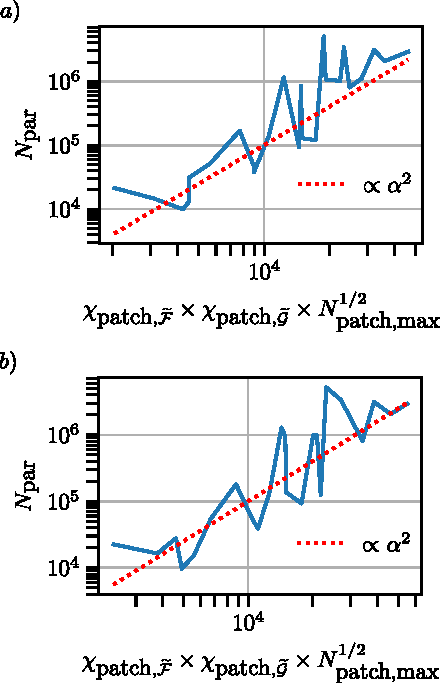
\includegraphics{figures/elemMulMemoryScaling.pdf}
    \caption{Total parameter count of the patched tensor \(\mF\mG\) versus the scaling variable from Eq.~\eqref{eq:newElemScalingApp}.  Solid lines: data (fused and interleaved orderings); dotted lines: expected scaling.}
    \label{fig:elemMulMemoryScaling}
\end{figure}



